\documentclass[a4paper, 10pt, final]{article}

\usepackage{a4wide}

\usepackage{charter}
\usepackage{verbatim}
\usepackage{amsfonts}
\usepackage{amsmath}
\usepackage{amsthm}
\usepackage{amssymb}
%\usepackage[integrals]{wasysym}
%\usepackage{mathrsfs}
%\usepackage[mathcal]{euscript}
\usepackage{listings}
\usepackage{graphicx}
\usepackage{multirow}
\usepackage{multicol}
\usepackage{hyperref}
\usepackage{float}
\usepackage[small,bf]{caption}
\usepackage{synttree}
%\usepackage{pst-node}
%\usepackage{xypic}
\usepackage[table]{xcolor}
\usepackage{subfig}
%\usepackage{ulem} %use \normalem after begin document
\usepackage[authoryear]{natbib}

% Settings
\parindent=5pt
\parskip=8pt plus 2pt minus 4pt
\lstset{language=Matlab, basicstyle=\scriptsize,
    showstringspaces=false, numbers=left, stepnumber=1, numberstyle=\tiny, frame=tb}


\title{Statistical Methods for Machine Learning \\ Mandatory Project 3}
\author{Kasper Steenstrup\\Michael Andersen\\Esben Skaarup}
\date{\today}

\hypersetup{
colorlinks,%
citecolor=black,%
filecolor=black,%
linkcolor=black,%
urlcolor=black,%
bookmarksopen=false,
pdftitle={Statistical Methods for Machine Learning - Mandatory Project 2},
pdfauthor={Kasper Steenstrup, Michael Andersen \& Esben Skaarup}
}

\begin{document}
\maketitle

\subsection*{Question 3.1}


\newpage
\subsection*{Question 3.2}

We calculated the eigenvalues and eigenvectors for use in the following subquestions.

\begin{figure}[!htbp]
  \centering
  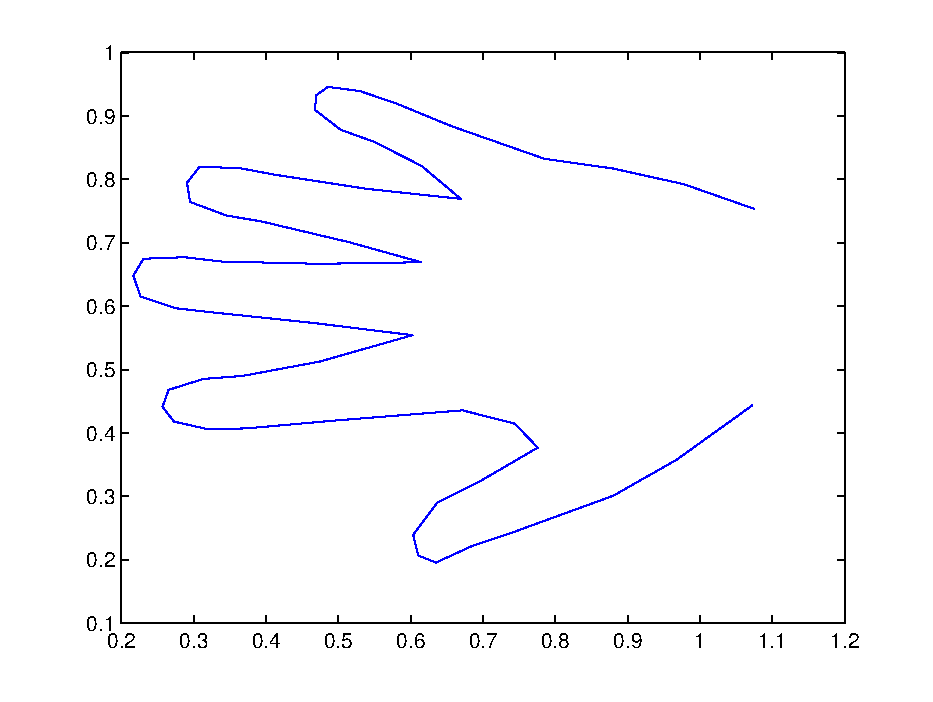
\includegraphics[width=0.85\textwidth]{./images/q32_mean}
  \caption{A hand consisting of the mean value of each data point.}
  \label{fig:q32_mean}
\end{figure}

\begin{itemize}
	\item
	First, we plot the mean values of each point.
	The results can be seen in figure \ref{fig:q32_mean}.
	The hand looks like a normal hand, with no distinct features, so it seems reasonable that this is the average of the hands.
	
	\item
	To visualize the number of components needed to capture the variations, we plotted the accumulated eigenvalues as a function of components used, seen in figure \ref{fig:q32_e}.
	6 components are needed to capture $95\%$ of the variation, and 11 are needed to capture $99\%$.
	Intuitively, it seems that around 5 of the components covers most of the variance, and around 10 covers almost all variation.
	Thus, all components except the first 10 (approximately) can be considered noise.
	
	\begin{figure}[!htbp]
	  \centering
	  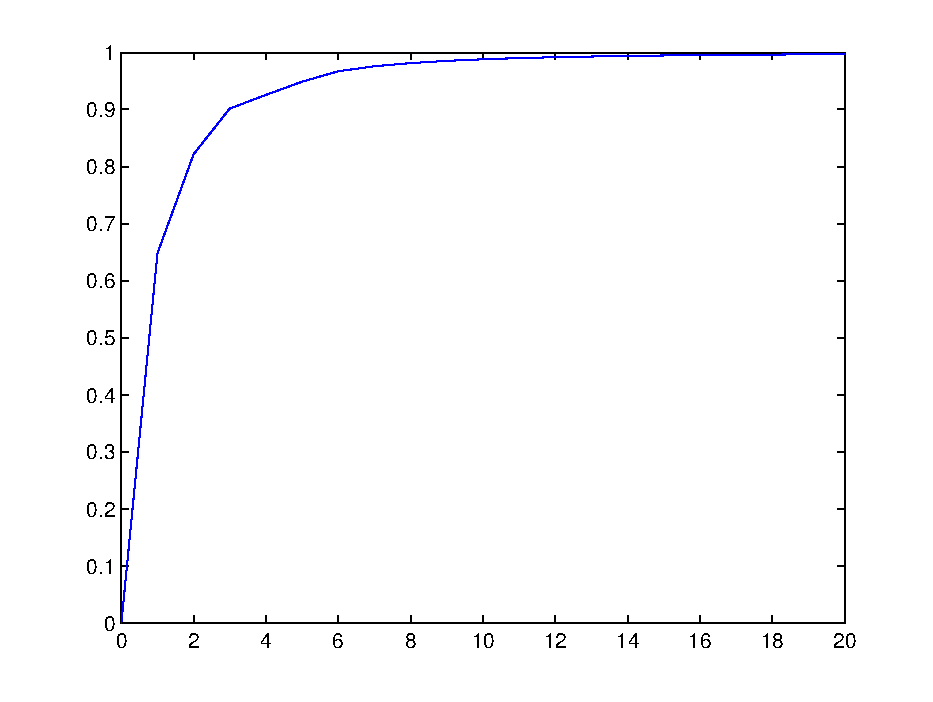
\includegraphics[width=0.85\textwidth]{./images/q32_e}
	  \caption{The amount of variance captured by different amounts of components.}
	  \label{fig:q32_e}
	\end{figure}
	
	\item
	To plot the meaning of the first principal component, we picked the largest eigenvector.
	We normalized the vector and added/subtracted it to/from the mean value (the average hand) to see how it affects it.
	The resulting plot can be seen in figure \ref{fig:q32_c}.
	It looks like the first principal component describes how much the fingers in the hand are spread out.
	This seems reasonable, as it is arguably the most distinct variation between the different hands.
	
	\begin{figure}[!htbp]
	  \centering
	  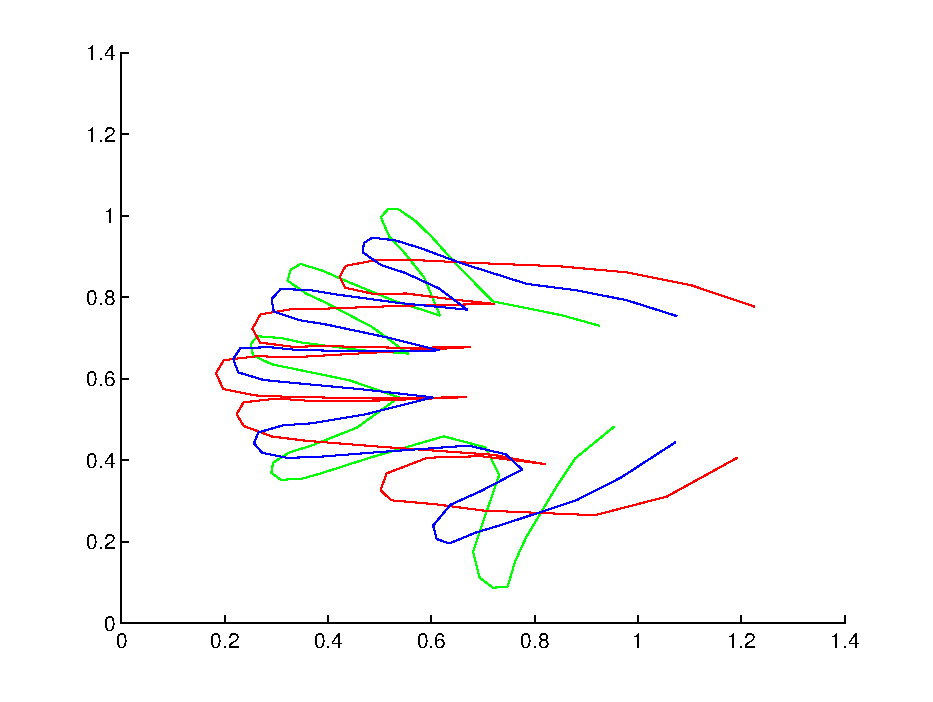
\includegraphics[width=0.85\textwidth]{./images/q32_c}
	  \caption{The mean hand (blue) and the same hand when the first principal component is added (red) and subtracted (green).}
	  \label{fig:q32_c}
	\end{figure}
	
	\item
	This analysis gave us the same kind of information as in question 3.1, but in much greater detail.
	Variating the first principal component shows the same pattern as the covariance plot (where one can see that the fingers can have varying distance to each other), but this analysis concluded how the variations happened together, where the former plot only hinted at it.
	Furthermore, this analysis taught us how many components are needed to describe the variance; a measure that could not be read from the analysis in question 3.1.
	
\end{itemize}

\newpage

\subsection*{Question 3.3}

\newpage
\subsection*{Question 3.4}

\newpage
\subsection*{Question 3.5}

\newpage
\subsection*{Question 3.6}

Plotting the cancer groups according to the first two principal
components can be seen in figure \ref{fig:q36pcs2}. Some of the cancer
groups seems to cluster nicely, especially \emph{MEL}, \emph{COL} and
\emph{LEU}. To some degree \emph{REN} also clusters nicely, but it
gets intermixed with some of the other cancer groups. \emph{BRE} looks
like it is spread all over, appearing both in \emph{MEL}, \emph{COL}
and the \emph{REN} cluster. This is using $k = 9$

\begin{figure}[!htbp]
  \centering 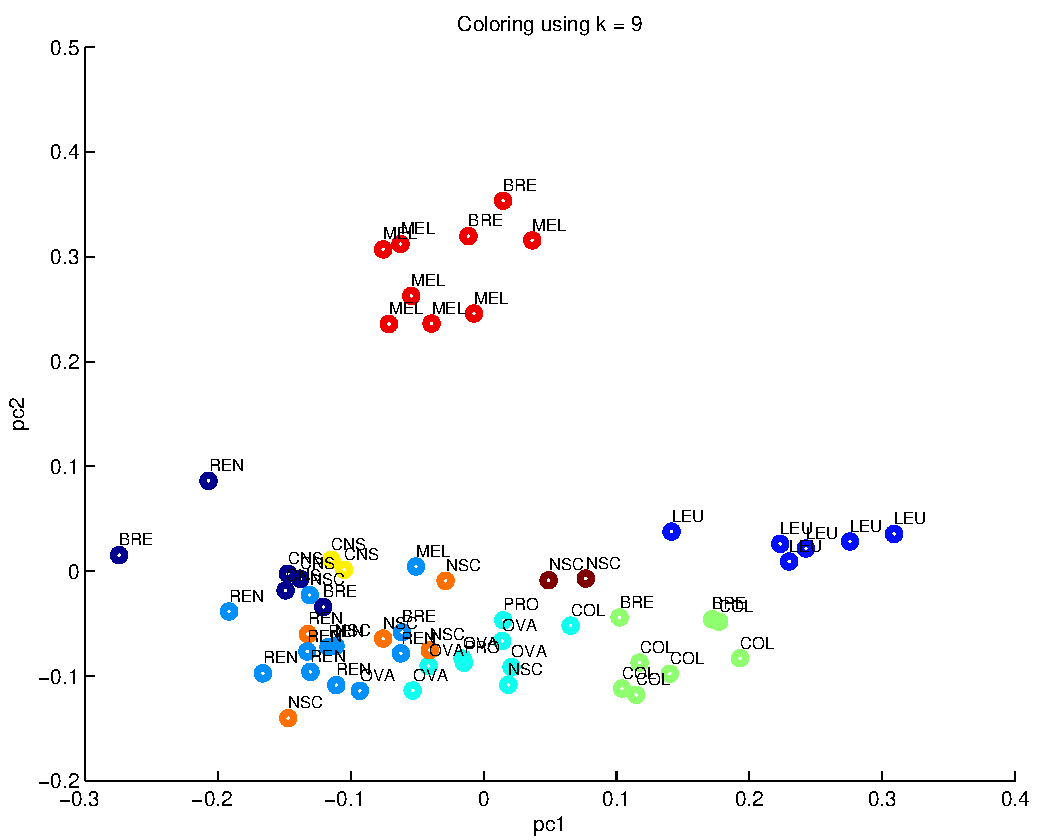
\includegraphics[width=0.95\textwidth]{./images/q36pcs2}
  \caption{2D plot according to pc$1$ and pc$2$ using k-means for
    coloring.}
  \label{fig:q36pcs2}
\end{figure}

\newpage

In figure \ref{fig:q36pcs3} can be seen using $k = 6$, the trend from
figure \ref{fig:q36pcs2} continues. \emph{NSC}, \emph{CNS}, \emph{OVA}
and \emph{BRE} seems intermixed in one big pile around pc$1$ $= -0.1$
and pc$2$ $= -0.05$. While the nicely clustered cancer groups from
figure \ref{fig:q36pcs2} again clusters nicely.

\begin{figure}[!htbp]
  \centering 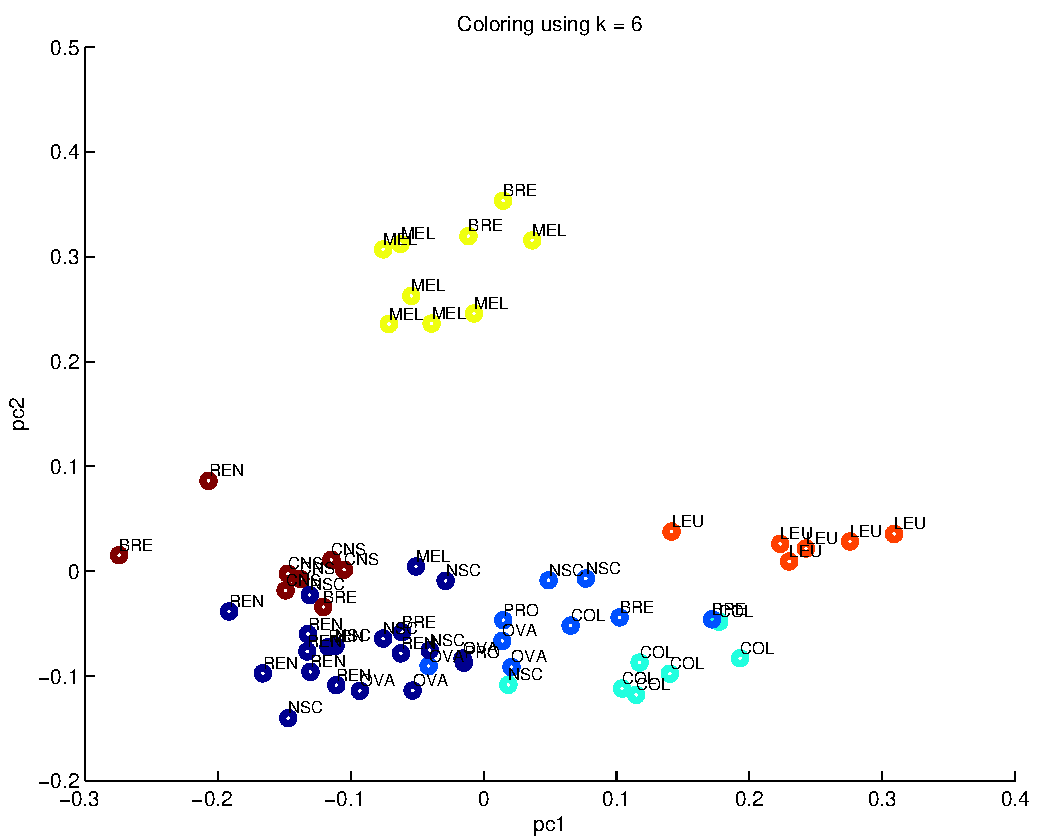
\includegraphics[width=0.95\textwidth]{./images/q36pcs3}
  \caption{2D plot according to pc$1$ and pc$2$ using k-means for
    coloring.}
  \label{fig:q36pcs3}
\end{figure}

\newpage

Here we now try to use the first three principal components to plot
the data in 3D. To see if we can find out why some of the cancer
groups where so intermixed in the two previuos figures. As we can see
the cancer groups are still intermixed. We had hoped that using the
three first principal components we would have been able to make a
better seperation of the cancer groups.

\begin{figure}[!htbp]
  \centering 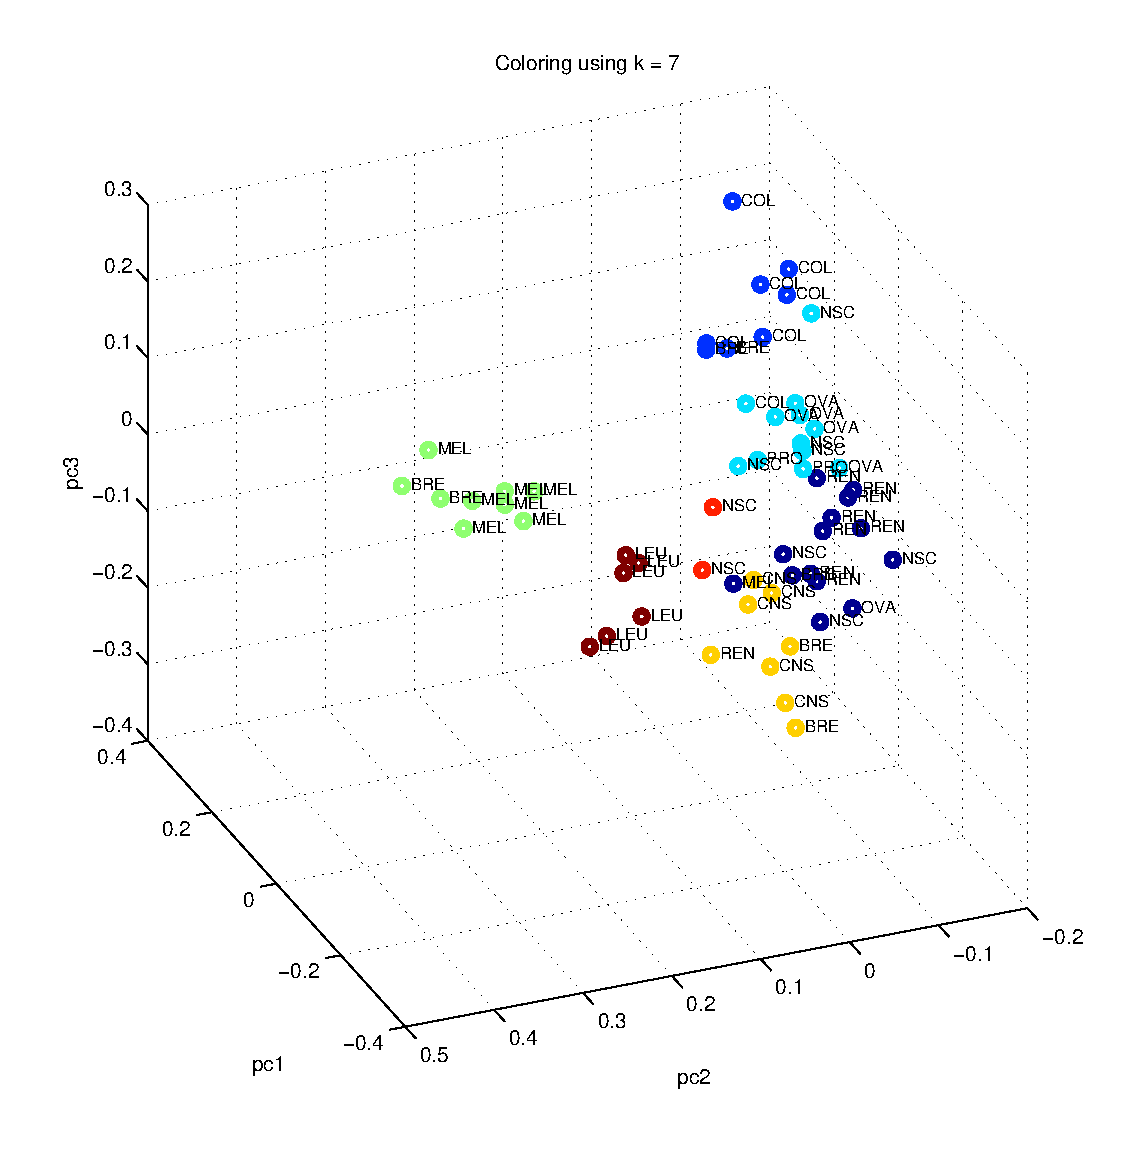
\includegraphics[width=0.95\textwidth]{./images/q36pcs4}
  \caption{3D plot according to pc$1$, pc$2$ and pc$3$ using k-means
    for coloring.}
  \label{fig:q36pcs4}
\end{figure}

From the above it seems like \emph{BRE} and \emph{NSC} are rather
heterogenous with its variance originating from other sources. And
with \emph{PRO} being homogenous with \emph{OVA}. Some of \emph{NSC}
(three cancer types) are also very much like \emph{OVA}.

We have tried varying the number of \emph{k} over the range $2$--$10$,
but the most optimal choise of \emph{k} seems to be somewhere around
$6$ or $7$. Too low and we do not get enough separation between the
different cancer group. Using too high a \emph{k} and we start
seperating similar cancer types.

\newpage
\subsection*{Question 3.7}
We are to estimate the density of the second principal component. From
the figure \ref{fig:q37histograms} we see various histograms with
different numbers of bins. Our best guess is around $12$ or $15$ bins
seems optimal, this depicts a mixture model with two modes. If we have
too small a number of bins we loose the ability to capture the real
underlying distribution, on the other hand if we choose to large a
number of bins we end up with a very spiky histogram that are too
noisy to see the real distribution. So one has to choose some
intermediate number of bins.

\begin{figure}[!htbp]
  \centering
  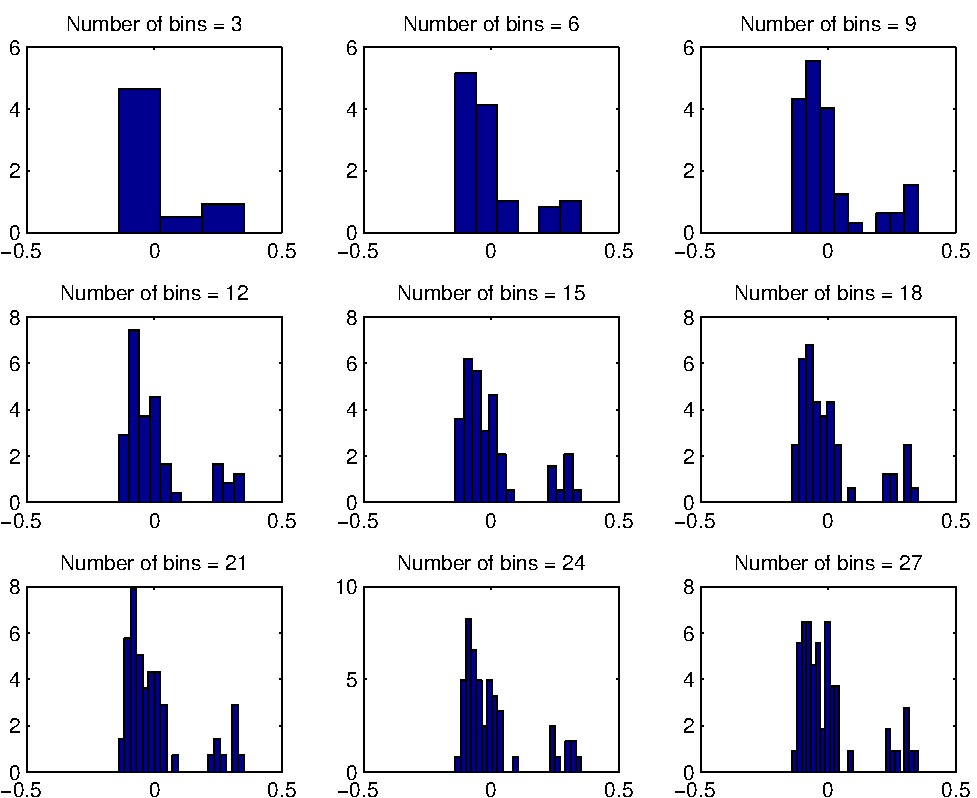
\includegraphics[width=0.85\textwidth]{./images/q37histograms}
  \caption{Shows histogram with various selections of bin numbers.}
  \label{fig:q37histograms}
\end{figure}

Next we are to try out kernel density estimator (kde), this can be
seen in figure \ref{fig:q37kde}. Again we see the same pattern as for
the histogram above. If we choose the bandwidth to be too low this
results in a very spiky structure where and choosing the bandwidth to
large we end up in the same situations as choosing a too small number
of bins. We loose the ability to capture the true form of the
underlying distribution. Some where between $0.03$ and $0.04$ seem to
be the optimal setting for capturing the two modes given by the second
principal component. Using automatic selection the code gives the
optimal bandwidth $0.0329$ which is very close to our best guess, this
can be seen in figure \ref{fig:q37kdeauto}. It is easy to see that
when setting the bandwidth to $>0.05$ the two modes within the data
starts to become one.

\begin{figure}[!htbp]
  \centering
  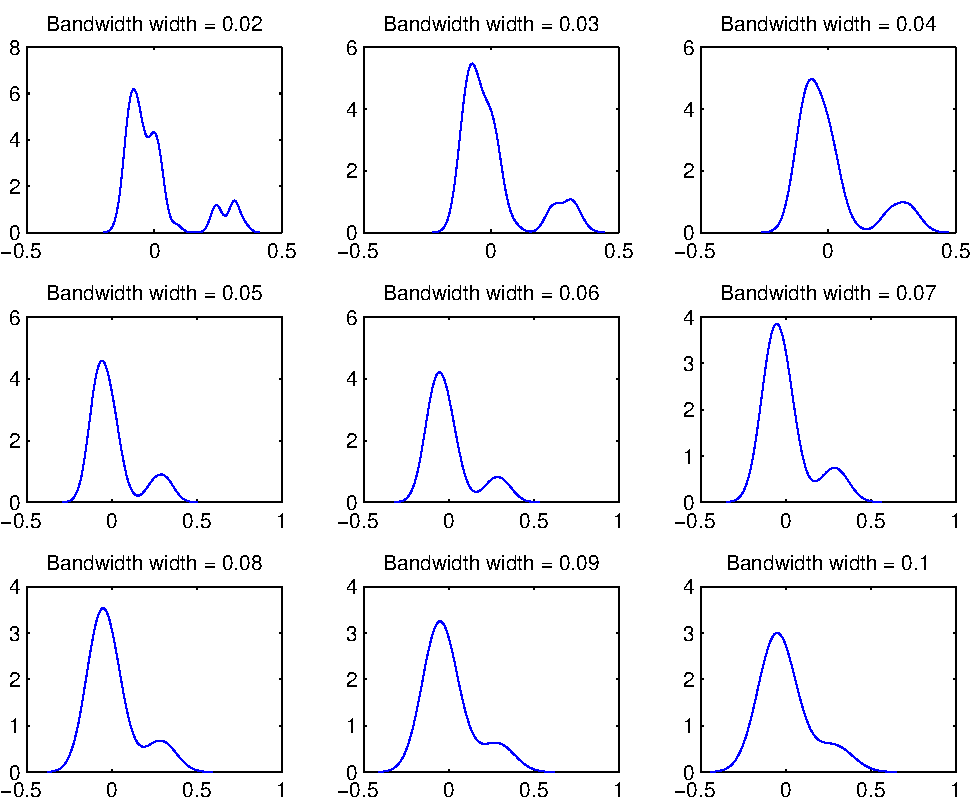
\includegraphics[width=0.85\textwidth]{./images/q37kde}
  \caption{Shows kernel density estimation for various selections of
    bandwidth.}
  \label{fig:q37kde}
\end{figure}

\begin{figure}[!htbp]
  \centering
  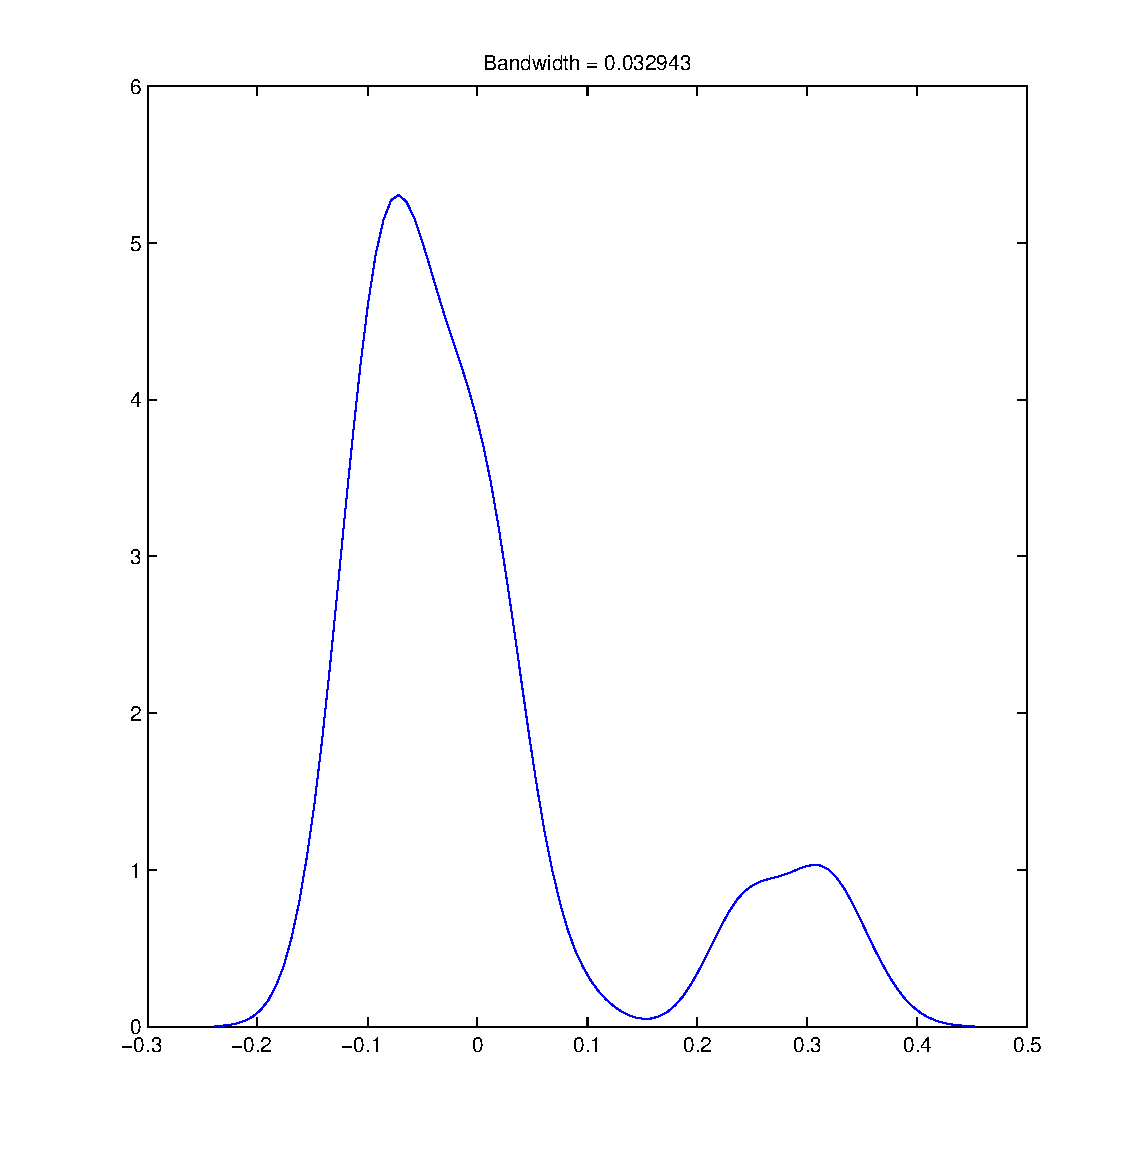
\includegraphics[width=0.65\textwidth]{./images/q37kdeauto}
  \caption{Shows kernel density estimation with automatic bandwidth
    selection.}
  \label{fig:q37kdeauto}
\end{figure}

\newpage

We are now to visualize $2d$ kernel density estimation based on the
first and second principal component. This is shown in figure
\ref{fig:q373dkde1} and \ref{fig:q373dkde2}. The figures shows the
same trends as the previously mentioned. Selecting the kernel
bandwidth too large causes the distribution to become too smooth,
thereby loosing the ability to captures the real form of the
distribution. Choosing the kernel bandwidth too small makes the
estimated distribution too spiky and noisy. So one has too choose some
intermediate. One this has to be noted, currently we select the same
bandwidth along both principal component. Better result can be
obtained by selecting individual bandwidth along the two different
axis.

\begin{figure}[!htbp]
  \centering
  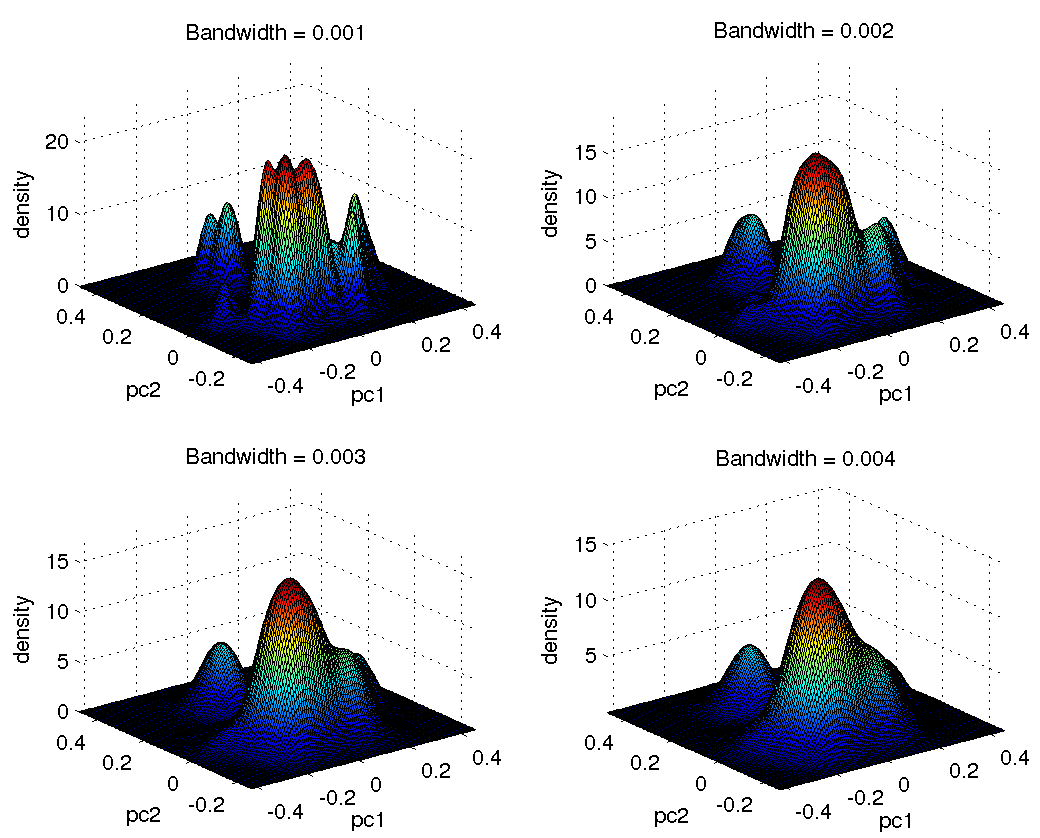
\includegraphics[width=1.0\textwidth]{./images/q373dkde1}
  \caption{Shows 2d kernel density estimations for various selections
    of bandwidth.}
  \label{fig:q373dkde1}
\end{figure}

\begin{figure}[!htbp]
  \centering
  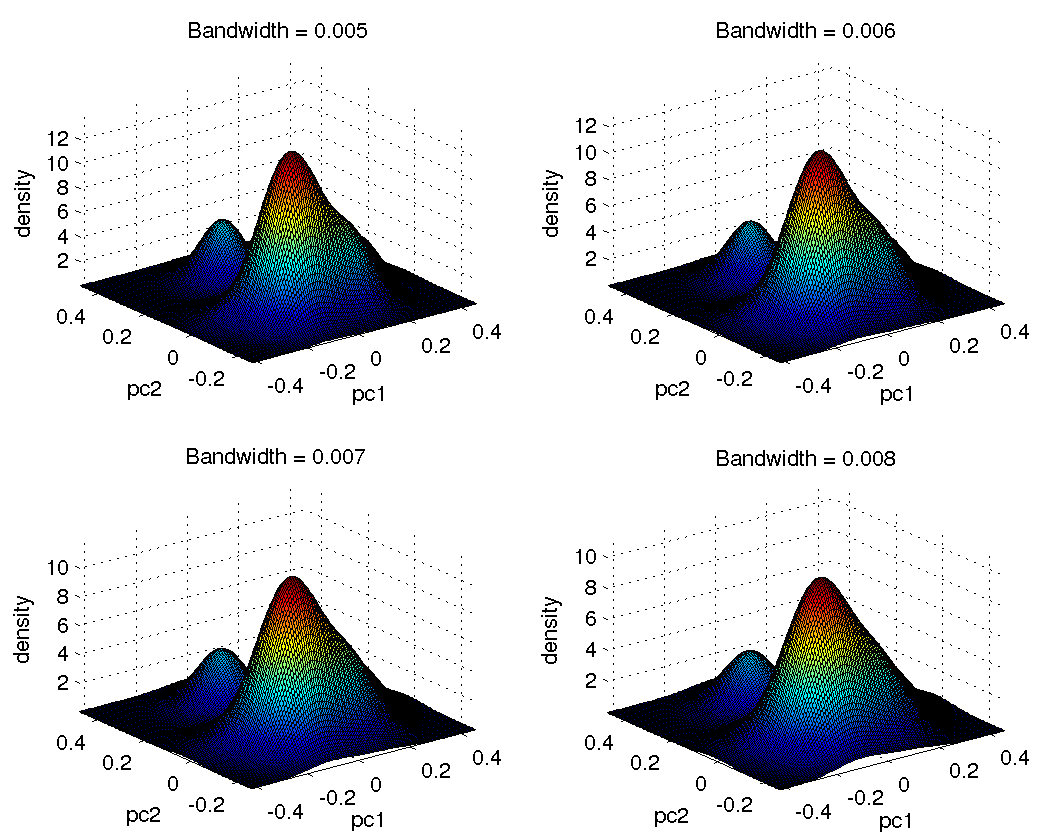
\includegraphics[width=1.0\textwidth]{./images/q373dkde2}
  \caption{Shows 2d kernel density estimations for various selections
    of bandwidth.}
  \label{fig:q373dkde2}
\end{figure}

\newpage

We are now to try out making density estimation using guassian mixture
model with various number of components. This is shown in figure
\ref{fig:q37mog}. When using two components, we are only able to
capture two of the modes within the two principal components. Using
three the result looks very reasonable, and this is our best guess at
what to use. Using four components, we starts to get $\delta$-spikes
where the component collapses onto a data point. This can be seen
around pc1 $= 0.2$ and pc2 $= 0.0$. The problem is even more visible
when using five components. We see that the 'top' of the density is
now around $60$ as opposed to $25$ when using three components.

\begin{figure}[!htbp]
  \centering
  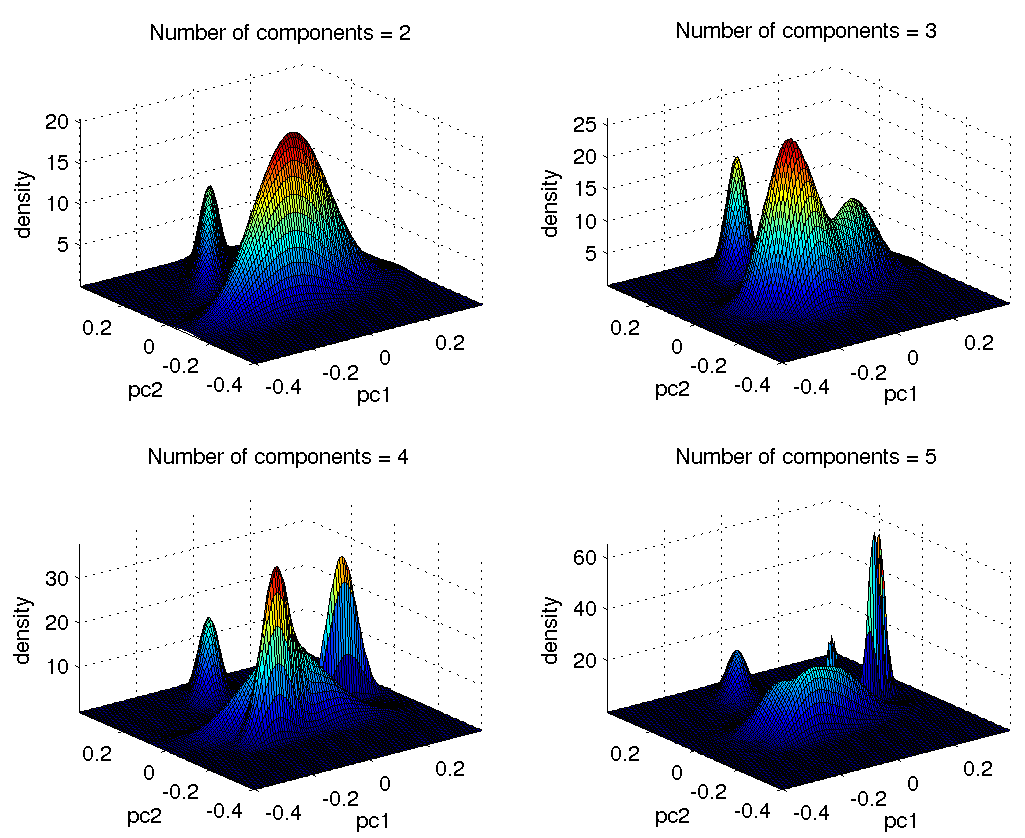
\includegraphics[width=0.95\textwidth]{./images/q37mog}
  \caption{Shows mixtures of gaussians for various selections of
    components in the model.}
  \label{fig:q37mog}
\end{figure}

It is unfortunately not possible to run \emph{gmdistribution.fit}
without specifying the number of components one wants to use within
the model. So it cannot be configured to automatic figure out what
number of components to use. We can instead try to use Akaike
Information Criterion for the estimated models, this idea is good
enough in theory. But as it turns out, it will always favor the one
with the largest number of components, even though this will be
severely over-fitted. As it turn out, is we let it run through
$1$--$11$ components, it will select $11$ and this is with the AIC
value: $-237.657405$, this is based on minimizing a negative log
likelihood function (More information can be found by searching for
\emph{aic} within the Matlab help system). A figure of the 'best'
number of components can be seen in figure \ref{fig:q37mogbest}, it is
very apperent that the model has collapsed onto a data points as it
peaks around $500$. And when selecting more that $11$ components the
programs breaks down with the following error: \emph{Ill-conditioned
  covariance error occurred in every replicate.}

\begin{figure}[!htbp]
  \centering
  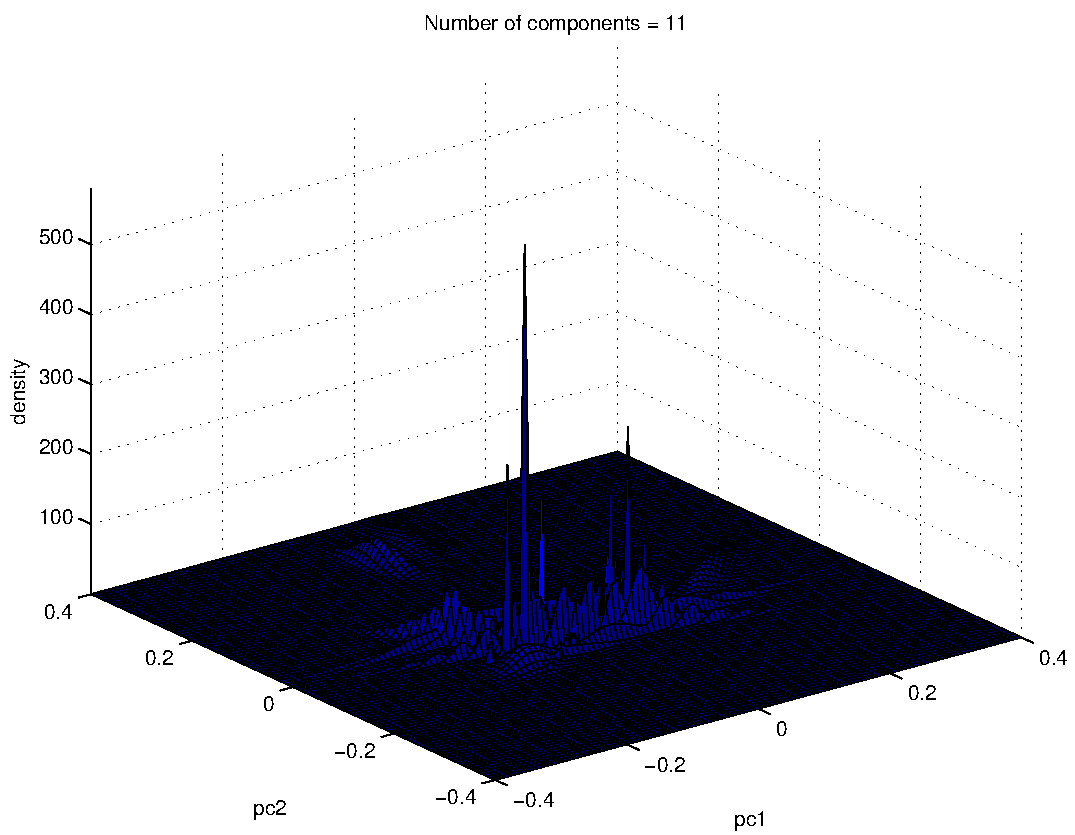
\includegraphics[width=0.95\textwidth]{./images/q37mogbest}
  \caption{Shows the 'best' mixtures of gaussians model.}
  \label{fig:q37mogbest}
\end{figure}

\newpage


%%%%%%%%%%%%%%%%%%%%%%%%%%%%%%%%%%%%%%%%%%%%%%%%%%%%%%%%%%%%%%%%%%%%
% Formal stuff

%\bibliographystyle{abbrvnat}
%\bibliography{bibliography}
%\addcontentsline{toc}{chapter}{Litteratur

\end{document}
